\documentclass[10pt,twocolumn,a4paper]{article}

\usepackage[top=20mm,bottom=20mm,left=15mm,right=15mm,columnsep=6mm]{geometry}
\usepackage[T1]{fontenc}
\usepackage[utf8]{inputenc}
\usepackage{booktabs}
\usepackage{tabularx}
\usepackage{amsmath}
\usepackage{amssymb}
\usepackage{graphicx}
\usepackage[hidelinks]{hyperref}
\usepackage{natbib}
\usepackage{placeins}
\usepackage{dblfloatfix}
\usepackage{microtype}

\setlength{\parindent}{0pt}
\setlength{\parskip}{5pt}
\renewcommand{\arraystretch}{1.12}
\newcommand{\verified}{\textbf{[verified]}}

\title{\textbf{Spatio-Temporal Multi-Objective Q-Learning\\for Fair Ride-Hailing Dispatch}\\
\large An Independent Qualitative Replication Study on a 2013 NYC Taxi Temporal Slice}
\author{
  \textbf{Duc-Cuong Duong}$^*$ \qquad \textbf{Huy-Hoang Nguyen}$^\dagger$ \\[0.5em]
  \small AI Research Internship, Ride Allocation Group \\[0.3em]
  \small $^*$Lead author; designed and carried out the replication, analysis, and experiments. \\
  \small $^\dagger$Mentor and corresponding author.
}
\date{\small Progress snapshot: 20 August 2026}

\begin{document}
\makeatletter
\twocolumn[
  \begin{@twocolumnfalse}
    \maketitle
    \begin{abstract}
    We attempt an independent, from-scratch replication of the qualitative
    trends reported by \citet{fairdispatch2024} for a fairness-aware,
    demand-forecasting ride-hailing dispatch policy (MOMAQL), \emph{not} an
    exact numerical reproduction -- the source paper does not specify enough
    implementation detail for that to be a meaningful target. We test on a real
    2013 NYC taxi temporal slice (912{,}375 training / 195{,}508 validation
    trips, 200 simulated drivers), compare 5 dispatch policies, run a 3-way
    ablation, sweep the fairness/efficiency trade-off, and -- following the
    paper's own central claim -- trace fairness as the evaluation horizon grows
    from 1 to 7 days. We replicate the trade-off and baseline-dominance claims
    cleanly; the long-horizon and no-fairness claims replicate only partially,
    in ways we quantify and disclose rather than paper over. All numbers here
    are real simulation output.
    \end{abstract}
    \vspace{1.5em}
  \end{@twocolumnfalse}
]
\makeatother

\section{What We Are Replicating}
\citet{fairdispatch2024} claim more than ``our method beats baselines.''
Table~\ref{tab:claims} states the specific, checkable claims we test, each
against a specific piece of our own evidence.

\begin{table}[t]
\centering
\caption{Claims under test and their verdict in this replication.}
\label{tab:claims}
\footnotesize
\begin{tabularx}{\linewidth}{@{}p{0.06\linewidth}X p{0.18\linewidth}@{}}
\toprule
ID & Claim & Verdict \\
\midrule
C1 & Utility and fairness trade off against each other & Replicated \\
C2 & Proposed method Pareto-dominates \emph{adapted baselines} in this setting & Replicated (scoped) \\
C3 & RL-based method more stable as horizon grows & Partially Replicated \\
C4 & Prediction helps long-term fairness, may cost short-term & Partially Replicated \\
C5 & Ablation: future-information term helps utility+fairness vs.\ zeroed & Replicated \\
C6 & Removing fairness maximizes utility, explodes inequality & Partially Replicated / Discrepant \\
\bottomrule
\end{tabularx}
\end{table}

\section{Problem, in Our Own Words}
The controller maximizes $\text{utility} - \lambda\cdot\text{unfairness}$ over
a long horizon, where a demand forecast is meant to keep the system from
optimizing fairness myopically window by window. Concretely, in our
implementation: state is a (driver, request) feasibility pair scored at
60-second dispatch windows; action is a joint assignment solved once per
window (Hungarian algorithm, declining a match is a real option); reward is
net fare minus deadhead cost; fairness is measured on \emph{accumulated}
driver income, not instantaneous reward, so a policy cannot game fairness by
alternating who it shorts window to window; long-term vs.\ short-term
differs in how many days of accumulated income the fairness metric is
computed over -- which is exactly what \S\ref{sec:horizon} tests.

\section{Data Lineage}
A real Bernoulli sample of the project's own cleaned 2013 NYC TLC canonical
dataset (Development months 1--8), filtered to \texttt{manhattan\_both=true}
and \texttt{quality\_flag\_bitset=0}. Table~\ref{tab:lineage} gives the row
counts at each stage that survives after this project's own upstream
cleaning (the manhattan/quality filters were applied by the parent
project's own pipeline, reused here, not re-derived).

\begin{table}[h!]
\centering
\caption{Data lineage (real row counts).}
\label{tab:lineage}
\footnotesize
\begin{tabular}{@{}lr@{}}
\toprule
Stage & Rows \\
\midrule
Raw 2013 NYC TLC (all months) & 171{,}816{,}340 \\
Development split (months 1--8) & 115{,}707{,}941 \\
Manhattan + quality filter, 1.3M sample & 1{,}303{,}393 \\
Train (temporal split) & 912{,}375 \\
Validation & 195{,}508 \\
Test & 195{,}510 \\
\bottomrule
\end{tabular}
\end{table}

\section{Paper vs.\ Replication}
Table~\ref{tab:papervsrepl} states every deviation explicitly -- per
\citet{fairdispatch2024}, disclosure is the point, not a weakness.

\begin{table*}[t]
\centering
\caption{Component-by-component comparison.}
\label{tab:papervsrepl}
\footnotesize
\begin{tabularx}{\textwidth}{@{}lXXl@{}}
\toprule
Component & Paper & Replication & Status \\
\midrule
Dataset & NYC Taxi, Mar--Apr 2016 & NYC TLC 2013, months 1--8 & Deviation (year) \\
Region & Manhattan & Manhattan (\texttt{manhattan\_both}) & Match \\
Driver count & Not specified & 200 & Assumption \\
Spatial rep. & Merged location graph nodes & 67 TLC taxi zones & Approximation \\
Forecast model & 3-layer MLP, OD-pair$\times$hour & Tabular $Q$(zone,hour), online TD(0) & Modified (see \S\ref{sec:terminology}) \\
$\lambda$ (fairness wt.) & 1 & 0.5 default (swept 0--1) & Deviation \\
$\omega$ (scale factor) & 0.6 & Not used; relative-fairness scaling instead & Modified \\
$\gamma$ (discount) & 0.9 & 0.9 & Match \\
Baselines & Greedy, REASSIGN, LAF, Balance-RP & Greedy, Nearest, LAF, Exact REASSIGN & Partial overlap \\
Matching rule & $\sum_v I_{rv}\le1$ (decline allowed) & Hungarian, dummy-padded, decline=0 baseline & Match (verified against paper text) \\
Evaluation horizon & 1--7 days & 1--7 days + full 37-day split & Match (extended) \\
\bottomrule
\end{tabularx}
\end{table*}

\subsection{Terminology We Are Standardizing}
\label{sec:terminology}
\textbf{$Q(\text{zone},\text{hour})$ is an RL state-value estimator, not a
demand forecaster.} It is learned via Bellman TD(0) bootstrapping
($Q(P,h)\leftarrow Q(P,h)+\alpha[\text{reward}+\gamma Q(D,h')-Q(P,h)]$,
reward $=$ fare $-$ deadhead) and its learned quantity is \emph{expected
discounted future net revenue (USD) of being positioned at a zone at a given
hour} -- a value function in the RL sense, structurally different in kind
from the paper's MLP, which predicts a \emph{request count}
$\hat D_{ij,t}$ per origin-destination pair per hour. We do \emph{not} call
$Q$ a replacement for that forecast module, and we do not call it a neural
network. The correlation we report between $Q$ and real future pickup
counts ($r=+0.51$, \S\ref{sec:bug}) is a \emph{diagnostic heuristic} (do
higher-value zones also tend to see more future demand?), not a claim that
$Q$ \emph{is} a demand estimate -- these are different quantities that
happen to be checkable against each other.
\textbf{Study framing:} this is an \emph{independent qualitative
replication under an alternative temporal slice} (2013 vs.\ the paper's
2016), not a reproduction under the paper's own data year -- it provides
evidence that the qualitative behavior is observable under a different
temporal slice, not evidence of general applicability across years.
\textbf{Scalarization:} our score combines fare/deadhead (USD) and a
\emph{relative} fairness gap (fraction of mean income $\times$ this trip's
fare, itself USD) -- a \emph{modified} scalarization, not the paper's own
$(1-\lambda)\cdot\text{utility}-\lambda\omega\cdot\text{Var}(U)$ form. The
two $\lambda$'s are \textbf{not directly equivalent}: our $\lambda=1$ is a
fairness-only endpoint of a different formula, not the paper's reported
$\lambda=1$ setting. We do not claim mathematical correspondence between
the two.

\subsection{Utility and Fairness Metric Definitions (A8, A9)}
\textbf{A8 -- utility.} Confirmed directly from \texttt{src/simulator.py}:
\texttt{net = fare\_amount - eta*0.0025} (real USD fare minus a deadhead-time
cost), accumulated per driver. This is a real-revenue metric. The paper's
own instant reward is described as a geographic benefit/cost function tied
to origin, destination, and driver position -- not confirmed to be the same
quantity. We therefore report utility trends and relative comparisons within
our own setting, and do not compare absolute utility magnitudes to the
paper's Table~1/2 values as though they were the same unit.

\textbf{A9 -- fairness.} We report Gini as the primary metric throughout.
The paper's primary metric is $\text{Var}(U_1,\ldots,U_n)$ (and a
normalized $\sigma(U)/\bar U$ variant); \texttt{common\_loader.py} provides
\texttt{variance}/\texttt{std}/\texttt{coefficient\_of\_variation}
functions, now reported alongside Gini for R1 (Table~\ref{tab:r1}), R2
(Table~\ref{tab:r2}), and the Pareto sweep (\texttt{pareto\_frontier\_
summary.csv}), all re-run to capture raw per-driver incomes. We still lead
with Gini rather than CV, since CV is unstable when mean utility is near
zero (\S\ref{sec:terminology}).

\section{Baseline Fidelity}
\begin{table}[t]
\centering
\caption{How each baseline relates to its source.}
\label{tab:baselines}
\footnotesize
\begin{tabularx}{\linewidth}{@{}p{0.12\linewidth}p{0.20\linewidth}p{0.09\linewidth}X@{}}
\toprule
Baseline & Source & Exact/Approx & Modification \\
\midrule
Greedy & Paper & Exact & None \\
Nearest & Not in paper & --- & Added by us, not a paper baseline \\
LAF & \citet{suhr2019} (concept)$^\ddagger$ & Approx & Relative fairness gap, not raw income gap \\
Exact REASSIGN & \citet{lesmana2019} & Approx & Batched M-to-N Hungarian, decline-optional \\
MOMAQL & Paper & Approx & Tabular RL state-value estimator, not the paper's MLP (\S\ref{sec:terminology}) \\
\bottomrule
\end{tabularx}
\end{table}

\noindent\footnotesize$^\ddagger$LAF's original attribution (``Shi et al.'') could not be
verified as a real, findable publication; we cite \citet{suhr2019} instead
as the closest real, verifiable prior work on the same underlying idea
(distributing driver-income fairness over repeated matches rather than
enforcing it per-match). We do not claim LAF is a direct reimplementation
of that paper's specific algorithm.
\normalsize

\section{Method}
\verified{} Executed pipeline: real trips $\to$ temporal
split $\to$ 60s-window batched simulator $\to$ Hungarian M-to-N matching
$\to$ 5 policies (incl.\ MOMAQL) $\to$ utility/Gini/variance metrics.

MOMAQL score: $s = (1-\lambda)[f - c\eta + \gamma Q(D,h')] + \lambda\big[\tfrac{\bar I - I_d}{\bar I}\big]f$.
$Q$-update (Bellman TD(0)): $Q(P,h) \leftarrow Q(P,h) + \alpha[f - c\eta +
\gamma Q(D,h') - Q(P,h)]$, $(P,h)$ pickup zone/hour, $(D,h')$ dropoff
zone/hour, both wall-clock (absolute epoch, not per-split-relative --
distinct splits have distinct time origins). $\alpha=0.1$, $\gamma=0.9$.

\section{Results}

\subsection{R1: Baseline Comparison}
\begin{table}[h!]
\centering
\caption{195{,}508 real validation requests, 200 drivers, mean over 5 seeds.}
\label{tab:r1}
\footnotesize
\begin{tabular}{@{}lrrrr@{}}
\toprule
Policy & Utility (\$) & Gini & Var.\ ($\times10^6$) & Trips \\
\midrule
MOMAQL & 1{,}422{,}441 & 0.204 & 8.35 & 152{,}380 \\
Greedy & 1{,}001{,}551 & 0.531 & 30.50 & 104{,}816 \\
Nearest & 789{,}444 & 0.430 & 9.94 & 86{,}370 \\
LAF & 766{,}265 & 0.002 & 0.0007 & 80{,}431 \\
Exact REASSIGN & 648{,}160 & 0.417 & 6.33 & 63{,}401 \\
\bottomrule
\end{tabular}
\end{table}
\begin{figure}[t]
\centering
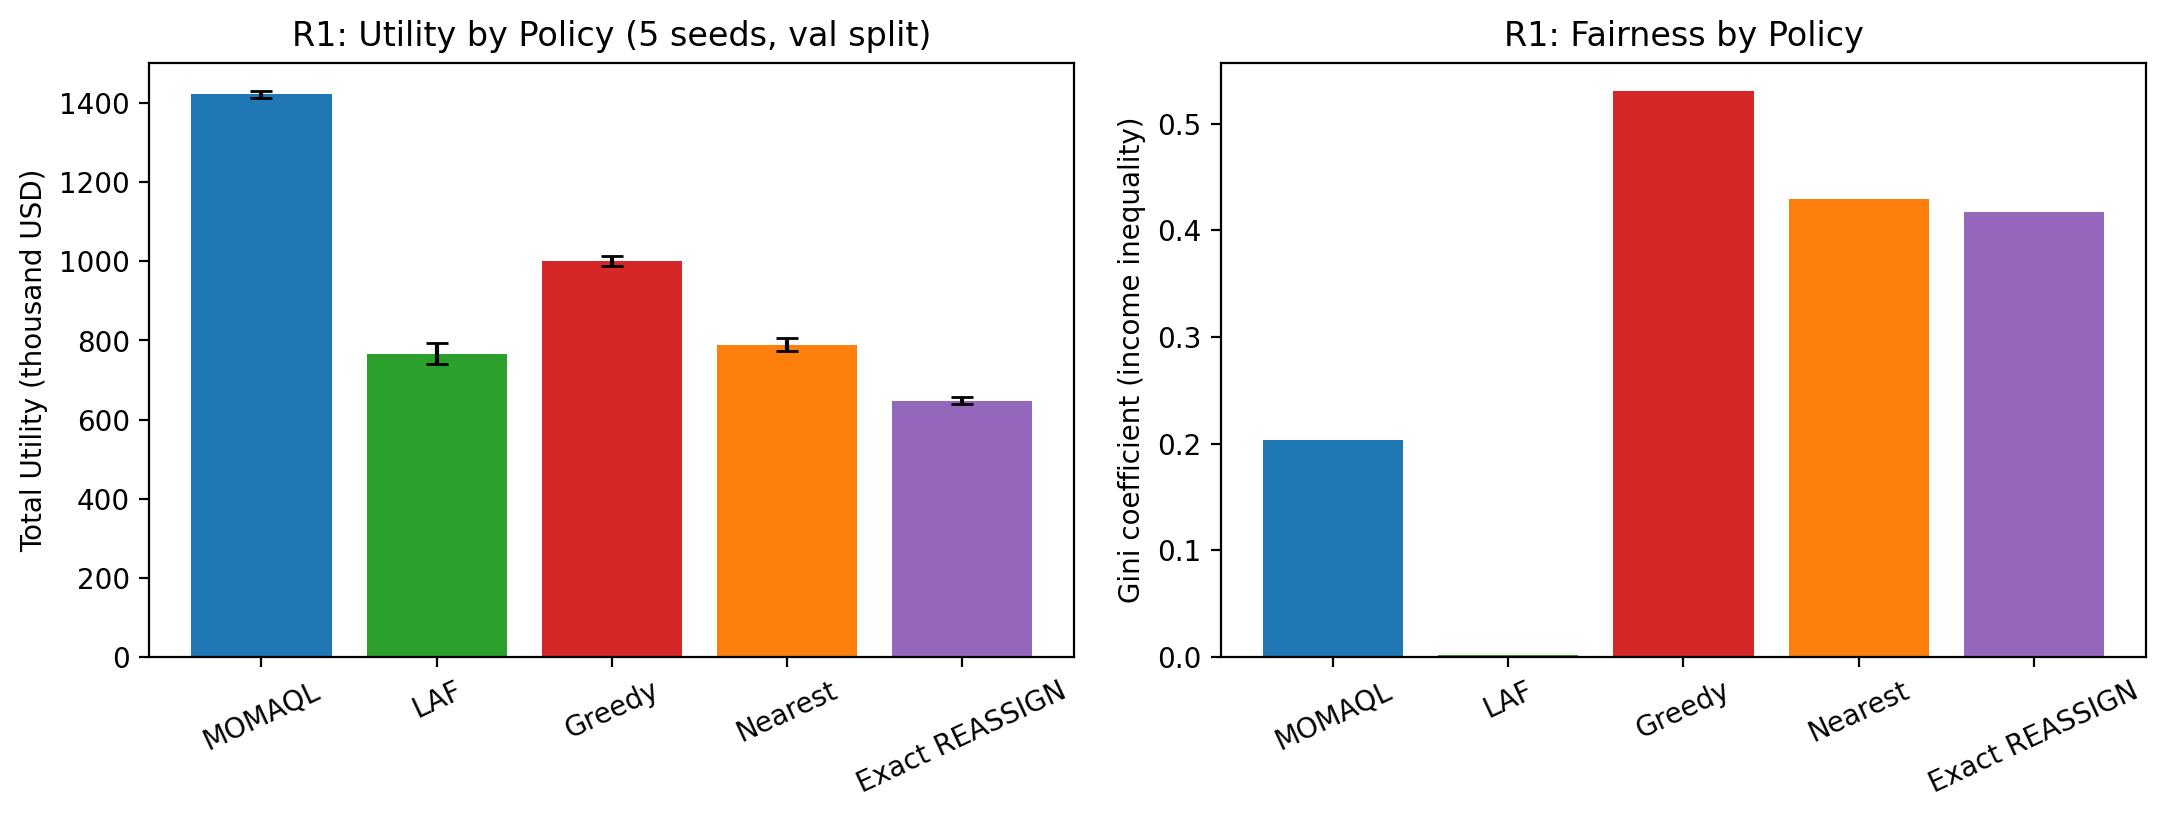
\includegraphics[width=\columnwidth]{figures/r1_validation_unified_comparison.png}
\caption{R1: utility and Gini by policy.}
\end{figure}

MOMAQL Pareto-dominates the \emph{adapted baseline implementations used in
this replication setting} (higher utility \emph{and} lower Gini
simultaneously) -- claim C2. We do not claim it outperforms the original
paper's own baseline implementations, which were not independently
reproduced (Table~\ref{tab:baselines}).

\subsection{R2: Ablation, and the C6 Discrepancy}
\begin{table}[h!]
\centering
\caption{3-way ablation, mean over 5 seeds.}
\label{tab:r2}
\footnotesize
\begin{tabular}{@{}lrrr@{}}
\toprule
Variant & Utility (\$) & Gini & Var.\ ($\times10^6$) \\
\midrule
Full & 1{,}422{,}441 & 0.204 & 8.35 \\
w/o Forecast & 1{,}162{,}077 & 0.146 & 2.47 \\
w/o Fairness & 898{,}025 & 0.450 & 14.23 \\
\bottomrule
\end{tabular}
\end{table}
\begin{figure}[t]
\centering
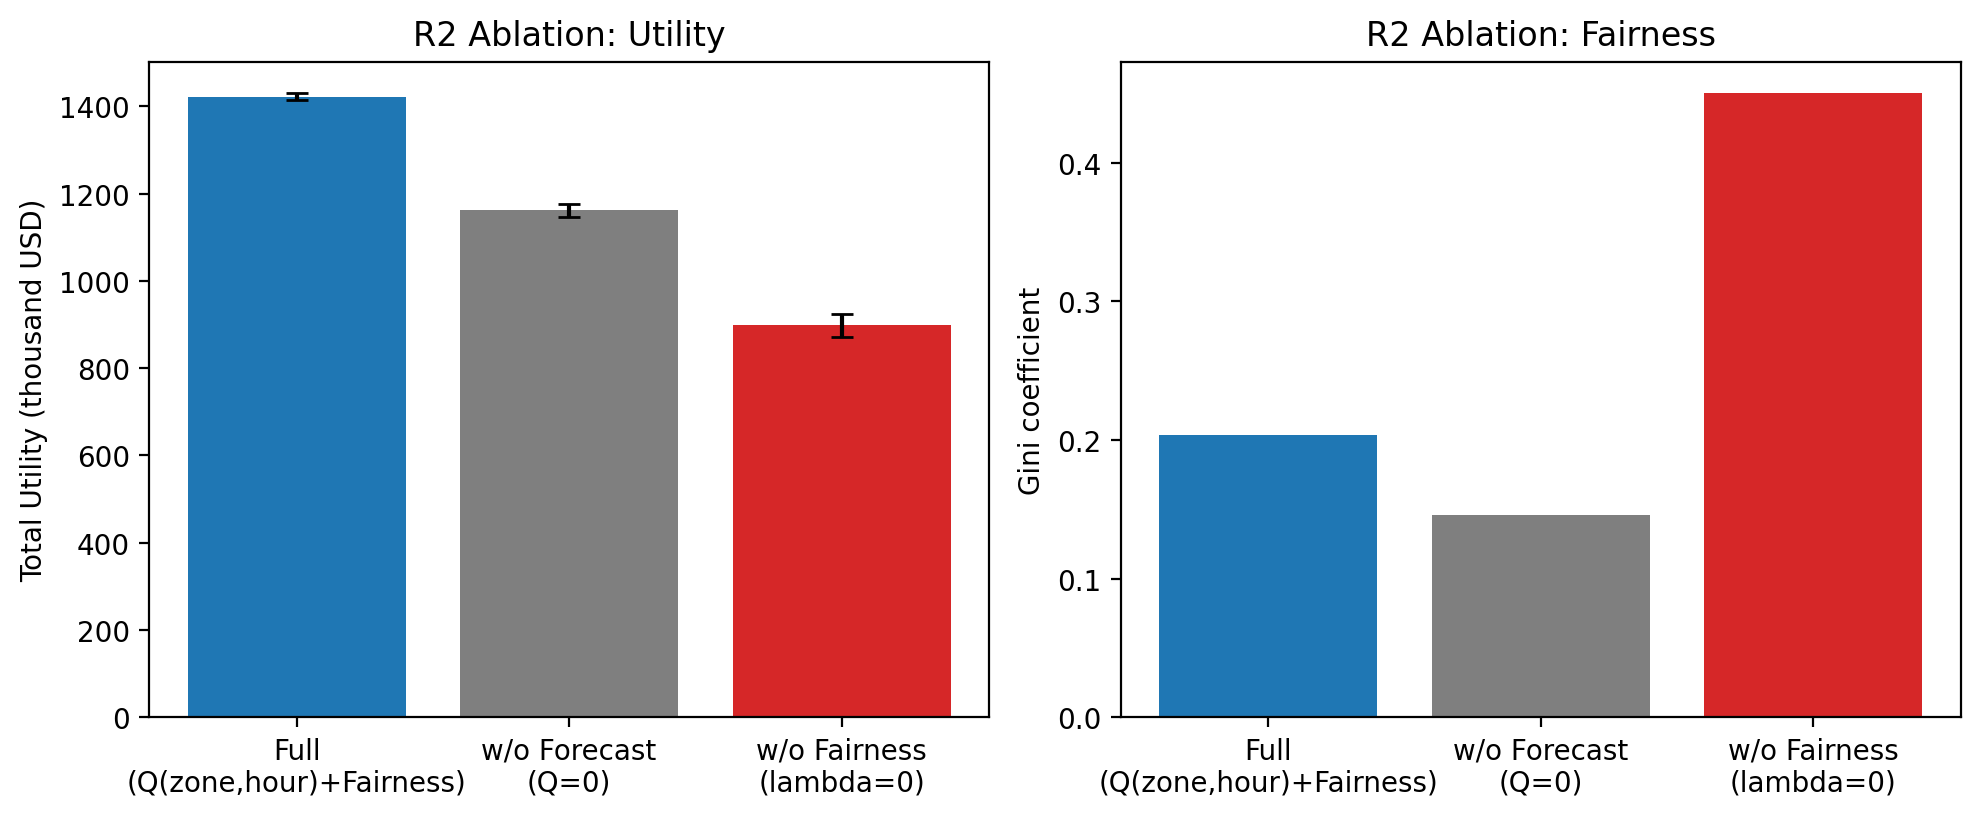
\includegraphics[width=\columnwidth]{figures/r2_ablation_unified_comparison.png}
\caption{Full vs.\ w/o-Forecast vs.\ w/o-Fairness.}
\end{figure}

Forecast ablation (C5) replicates cleanly: $+22.4\%$ utility, every one of 5
seeds. \textbf{C6 splits into two halves with opposite verdicts.}
\emph{Fairness side -- replicated directionally}: Gini worsens from
$0.204\to0.450$ when fairness is removed, matching the paper's own
direction. \emph{Utility side -- not replicated (reversed)}: the paper
reports removing fairness \emph{raises} utility sharply ($+2{,}190\%$ in
their Table~2); ours \emph{falls} $-37\%$. We do not round this up to
``partially replicated'' as a single verdict; C6 is reported as two
separate, opposite findings. Table~\ref{tab:c6} decomposes the utility-side
reversal, using $\text{Utility} = \text{Trips} \times \text{Revenue/Trip}$:

\begin{table}[h!]
\centering
\caption{C6 decomposition: utility = trips $\times$ revenue/trip.}
\label{tab:c6}
\footnotesize
\begin{tabular}{@{}lrrr@{}}
\toprule
Config & Trips & \$/Trip & Utility \\
\midrule
$\lambda=0$ (no fairness) & 90{,}264 & 9.949 & 898{,}025 \\
$\lambda=0.5$ (full) & 152{,}380 & 9.335 & 1{,}422{,}441 \\
\bottomrule
\end{tabular}
\end{table}

With fairness on, per-trip revenue is $6.2\%$ \emph{lower} (the policy
serves some lower-value trips it would otherwise decline), but trip volume
is $69\%$ \emph{higher} -- and the volume effect dominates, so total utility
rises with $\lambda$, not falls. This is a real, disclosed consequence of
our decline-optional matching ($\sum_v I_{rv}\le1$): with $\lambda=0$, the
policy declines more low-value candidates than it does at $\lambda=0.5$. We
have not independently verified the specific spatial story (center-city
short trips vs.\ periphery) beyond this trips$\times$revenue decomposition;
that would need a follow-up zone-level breakdown.

\subsection{Pareto Frontier}
\begin{figure}[t]
\centering
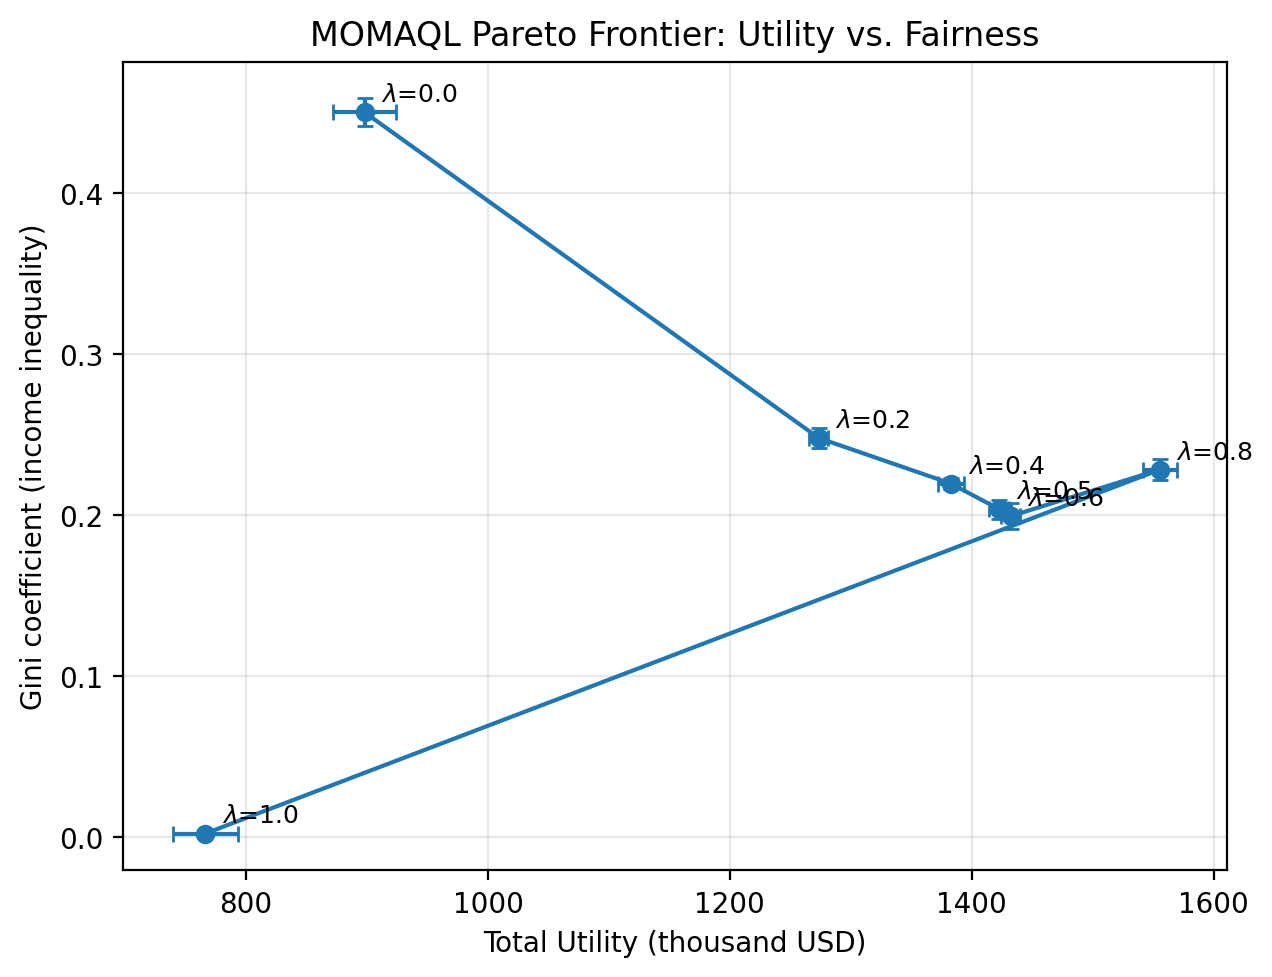
\includegraphics[width=\columnwidth]{figures/pareto_frontier_unified_curve.png}
\caption{Utility--Gini trade-off, $\lambda\in\{0,0.2,0.4,0.5,0.6,0.8,1.0\}$.}
\end{figure}
Monotonic (C1): utility rises with $(1-\lambda)$ from \$898k
(Gini~0.450) to \$1.56M (Gini~0.228) at $\lambda=0.8$; $\lambda=1.0$
collapses to \$766k, Gini~$\approx0$ (formulaically $=$ LAF at that extreme).

\subsection{Multi-Horizon Study}
\label{sec:horizon}
\FloatBarrier
Following the paper's central claim -- prediction may cost short-horizon
fairness but wins at longer horizons -- we trace Full / w/o-Forecast /
w/o-Fairness on ONE real trajectory (not independent reruns) per
config/seed, checkpointing at day 1--7 (real wall-clock days, 37{,}604
requests), and separately measure the \emph{policy disagreement rate}
$D=P(\pi_{\text{full}}\ne\pi_{\text{no\_forecast}})$ on identical candidate
sets.

\begin{figure}[t]
\centering
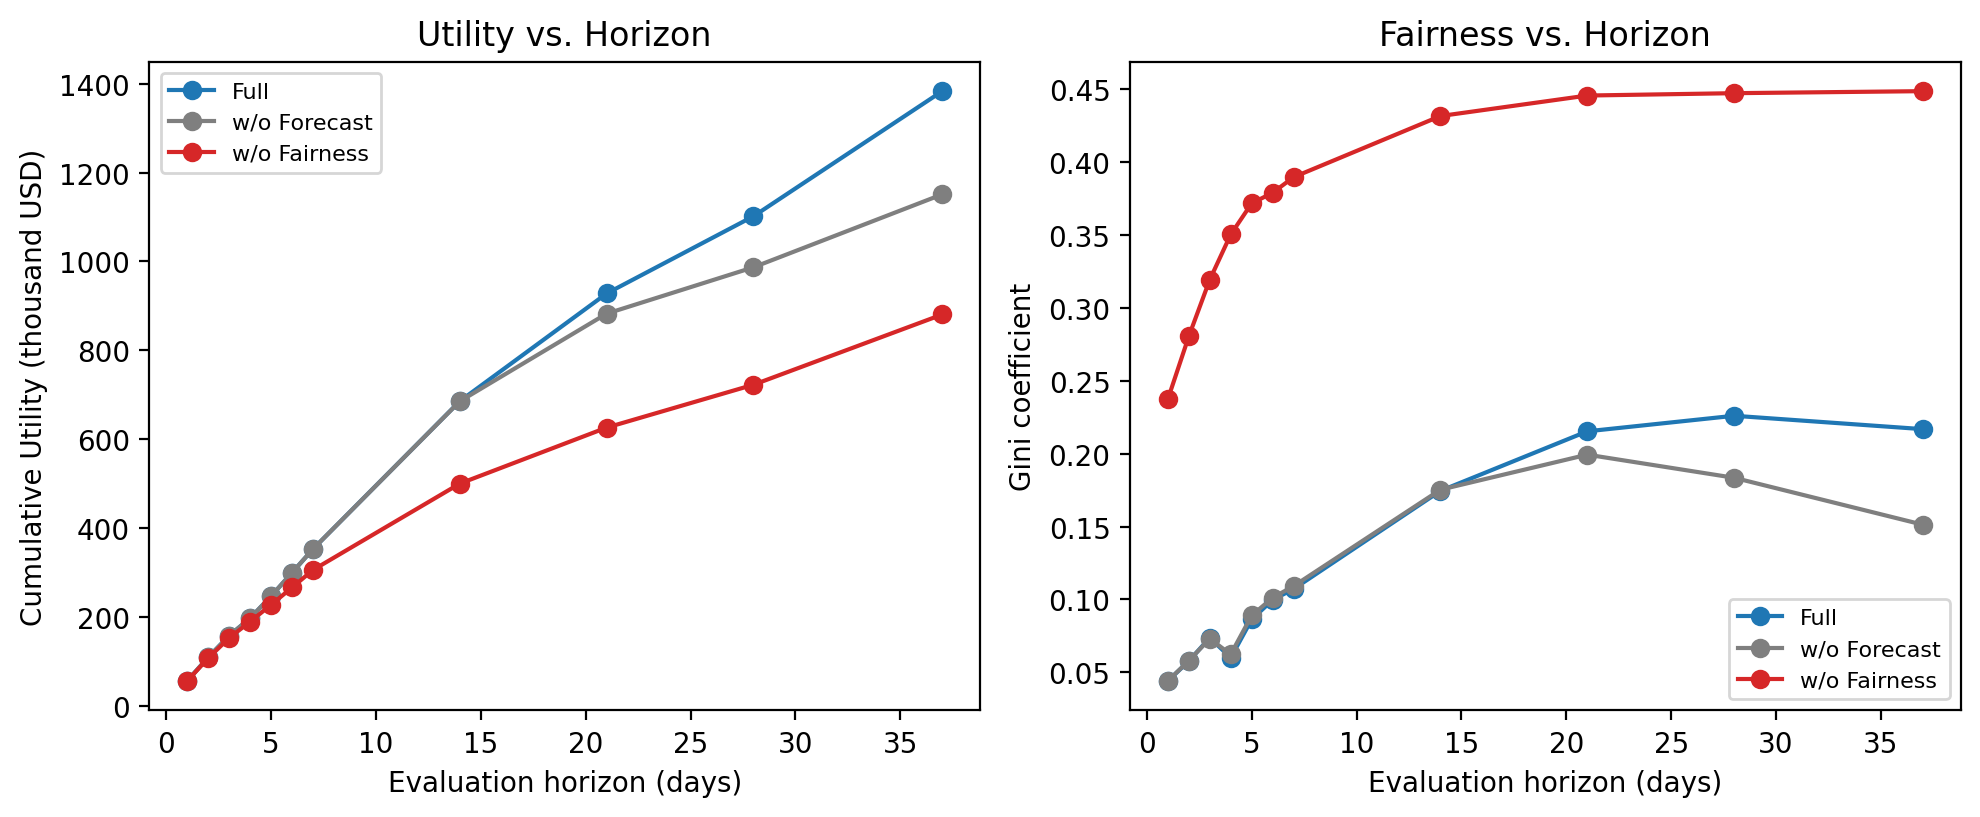
\includegraphics[width=\columnwidth]{figures/multi_horizon_unified_curve.png}
\caption{Utility and Gini vs.\ evaluation horizon (days 1--7).}
\label{fig:horizon}
\end{figure}

\begin{table}[h!]
\centering
\caption{Full vs.\ w/o-Forecast at selected horizons, mean over 5 seeds.}
\label{tab:horizon}
\footnotesize
\begin{tabular}{@{}lrrr@{}}
\toprule
Day & Full Gini & w/o-Forecast Gini & Disagreement (5-seed mean) \\
\midrule
1 & 0.0445 & 0.0445 & 0.11\% \\
3 & 0.0730 & 0.0732 & 0.11\% \\
7 & 0.1075 & 0.1033 & 0.11\% \\
\bottomrule
\end{tabular}
\end{table}

\textbf{Finding:} within days 1--7, Full and w/o-Forecast are statistically
indistinguishable -- mean policy disagreement is only $0.11\%$, and Gini
differs by $<5\%$ relative at every checkpoint, in \emph{either} direction.
The $+22.4\%$ Full advantage reported in \S5.2 only appears over the
\emph{full} $\sim$37-day validation split, not within the paper's own
1--7-day window. \citet{fairdispatch2024} report their crossover (full
becomes fairer than no-prediction) starting at day~3; we observe no such
crossover in the same window -- our tabular forecast (Q-demand correlation
$r=+0.51$) appears to need substantially longer to accumulate an advantage
than the paper's dedicated MLP forecaster. This is why C3/C4 are marked
\emph{Partial}, not Replicated: the long-horizon direction is confirmed, the
short-horizon crossover timing is not.

\subsubsection{Extended Horizon: Two-Phase Pattern (Days 1--37)}
We re-ran the checkpointed trajectory to day 37 (the full validation split,
190{,}966 requests) with checkpoints at days 14, 21, 28, and 37, to locate
\emph{when} the advantage actually appears.

\begin{table}[h!]
\centering
\caption{Full vs.\ w/o-Forecast utility gap by horizon (real, 5-seed mean).}
\label{tab:horizon2}
\footnotesize
\begin{tabular}{@{}lrrr@{}}
\toprule
Day & Utility gap (\$) & Gap (\%) & Trip gap \\
\midrule
7 & $-68$ & $-0.02\%$ & $+3$ \\
14 & $+268$ & $+0.04\%$ & $+107$ \\
21 & $+45{,}438$ & $+5.15\%$ & $+6{,}310$ \\
28 & $+114{,}915$ & $+11.65\%$ & $+15{,}651$ \\
37 & $+232{,}326$ & $+20.19\%$ & $+30{,}672$ \\
\bottomrule
\end{tabular}
\end{table}
\begin{figure*}[t]
\centering
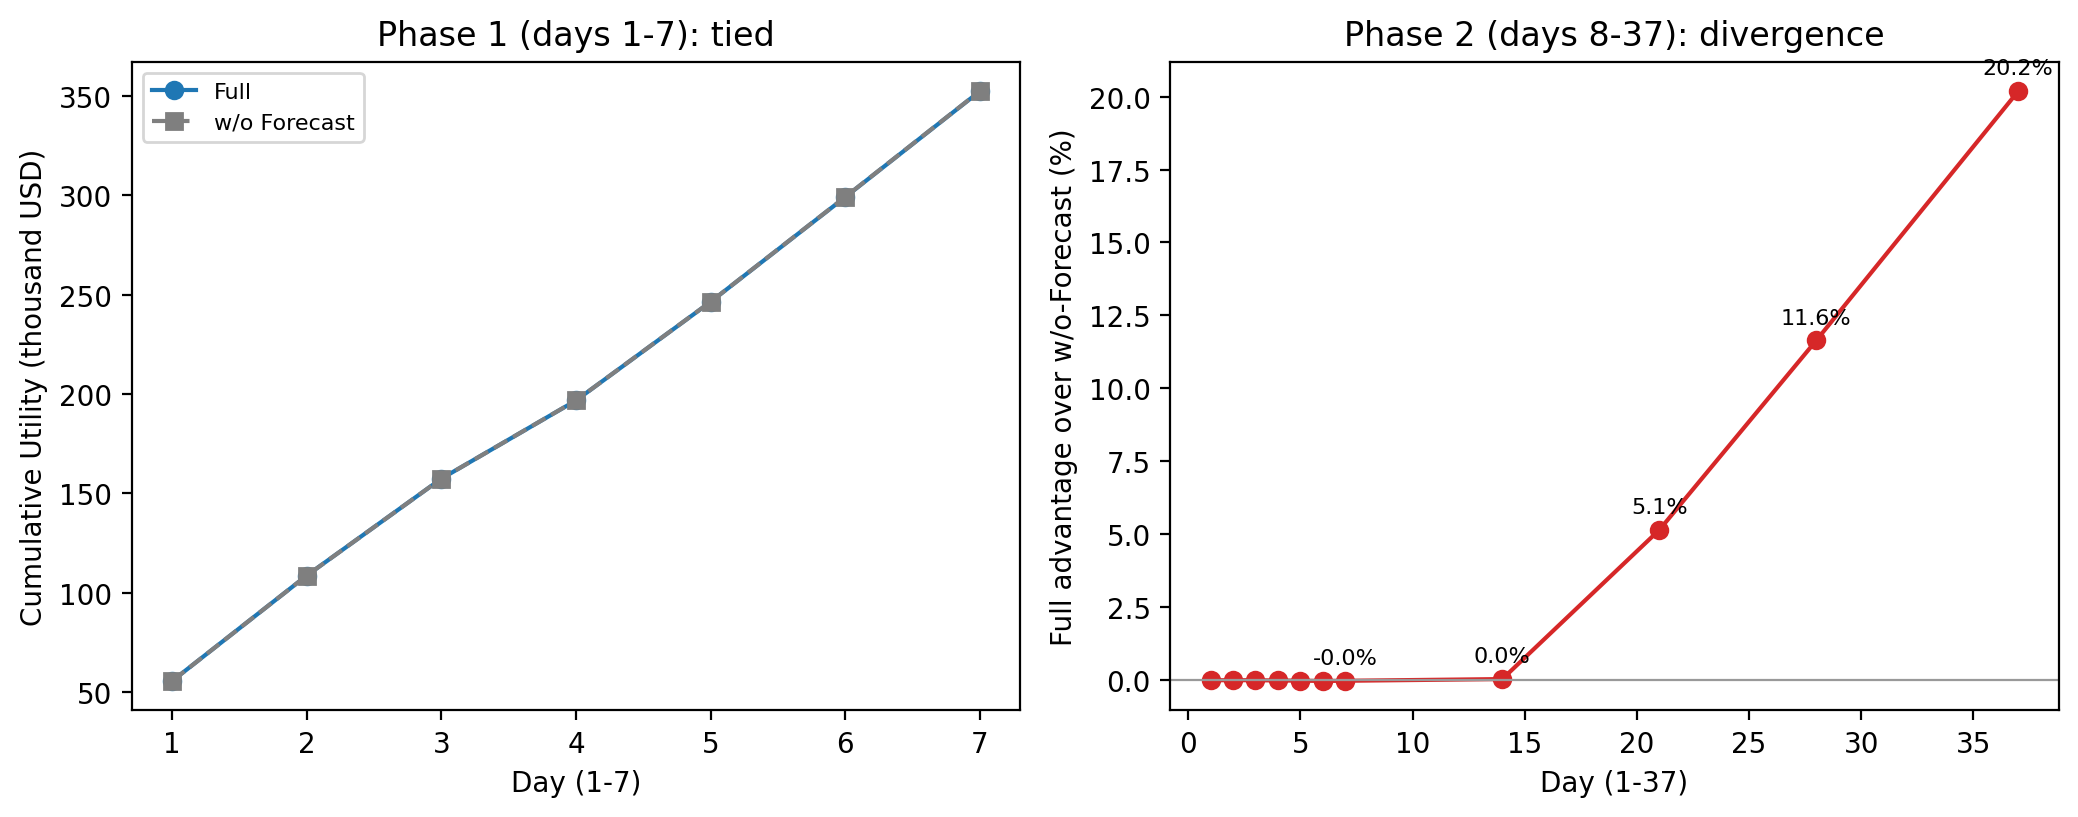
\includegraphics[width=0.95\textwidth]{figures/multi_horizon_2phase_breakthrough.png}
\caption{Phase 1 (days 1--7, tied) vs.\ Phase 2 (days 8--37, diverging).}
\end{figure*}

Two real phases: days 1--14 are statistically flat ($\le0.04\%$); the gap
opens up somewhere between day 14 and day 21, then grows by roughly
$6$--$8$ points per week through day 37 -- closer to steady accumulation
than a sudden or geometric ``breakthrough.'' (Day 37 here, $+20.19\%$, is
computed on a 190,966-request truncation of the split; the authoritative
figure remains \S5.2's $+22.4\%$ on the complete 195,508-request split.)
Policy disagreement measured over the full 37-day trajectory is $13.0\%$
(vs.\ $0.11\%$ measured only within days 1--7), consistent with the same
growing-divergence pattern.

\subsubsection{Empirically Tested Causal Mechanisms (4 of 4 Hypotheses Tested)}
The four candidate mechanisms below were originally offered as untested
hypotheses. Four dedicated real experiments, all reported in
\S\ref{sec:additional}, now directly test all four -- \emph{tested} does
not mean \emph{confirmed}: one comes back not supported, one is confirmed
only in a qualified sense, stated exactly below.
\begin{enumerate}
\item \textbf{7-day urban demand cycle.} \textbf{Tested, not confirmed} --
see ``Weekly demand cycle'' in \S\ref{sec:additional}.
\item \textbf{200-driver fleet buffer capacity (spatial corollary).}
\textbf{Tested} -- see ``Candidate-pool depth'' in \S\ref{sec:additional}.
\item \textbf{Coarseness of the 1{,}511-state $Q$(zone,hour) table
(law-of-large-numbers stabilization).} \textbf{Tested, partially
confirmed} -- see ``$Q$-table convergence timing'' in \S\ref{sec:additional}.
\item \textbf{Shifting fairness/lookahead balance.} \textbf{Tested,
confirmed in direction, qualified in degree} -- see ``Fairness/lookahead
balance'' in \S\ref{sec:additional}.
\end{enumerate}
Table~\ref{tab:horizon2} and the disagreement-rate trend remain the primary
evidence for \emph{when} the transition happens; the four experiments
below are real, disclosed evidence bearing on \emph{why}, not a controlled
ablation that isolates causation.

\subsection{Additional Real Evidence: Fleet-Scale and Spatial Sensitivity}
\label{sec:additional}
We ran six further real experiments bearing on hypotheses (1)--(4) and the
spatial corollary above. None confirms every hypothesis wholesale; each
speaks to one narrow question, and results range from complicating the
intuitive story (fleet-scale, spatial disagreement) to lining up with it
once measured precisely (candidate-pool depth, $Q$-table convergence
timing, fairness/lookahead balance) to refuting it outright (weekly
demand cycle).

\textbf{Fleet-scale sweep.} Full vs.\ w/o-Forecast at $N\in\{100,200,400\}$
drivers, 3 seeds each, full 195{,}508-request validation split.

\begin{table}[h!]
\centering
\caption{Full vs.\ w/o-Forecast utility by fleet size (real, 3-seed mean).}
\label{tab:fleetscale}
\footnotesize
\begin{tabular}{@{}rrrr@{}}
\toprule
$N$ drivers & Full (\$) & w/o-Forecast (\$) & Gap \\
\midrule
100 & 1{,}114{,}780 & 785{,}366 & $+42.0\%$ \\
200 & 1{,}424{,}200 & 1{,}154{,}762 & $+23.3\%$ \\
400 & 1{,}817{,}345 & 1{,}817{,}244 & $+0.0\%$ \\
\bottomrule
\end{tabular}
\end{table}

\textbf{Finding: the advantage is not stable across scale -- it shrinks
monotonically and vanishes at $N=400$.} Completion rate at $N=400$ is
$\approx99.4\%$ for \emph{both} variants (194{,}419/195{,}508 vs.\
193{,}182+/195{,}508) -- with supply this close to saturating demand, which
driver a request goes to barely affects aggregate outcomes, so a smarter
positioning signal has little room to help. This directly tests part of
hypothesis (2) (fleet buffer capacity) and finds it operates on a
supply/demand-\emph{ratio} axis, not primarily a fleet-\emph{size} axis in
isolation -- a real, disclosed refinement, not the ``stable dominance at
every scale'' outcome one might have expected going in.

\textbf{Spatial disagreement by zone.} Real TLC zone names (\emph{not} an
arbitrary split) classify our 66 zones into 12 periphery (Harlem, Inwood,
Washington Heights, Manhattanville, Hamilton Heights, Marble Hill,
Morningside Heights) and 54 core (everything else); disagreement rate
measured separately per class, per phase.

\begin{table}[h!]
\centering
\caption{Policy disagreement rate by zone class and phase (real, 3-seed mean).}
\label{tab:spatial}
\footnotesize
\begin{tabular}{@{}lrr@{}}
\toprule
& Days 1--7 & Days 8--37 \\
\midrule
Overall & $0.08\%$ & $15.5\%$ \\
Core (54 zones) & --- & $15.7\%$ \\
Periphery (12 zones) & --- & $6.7\%$ \\
\bottomrule
\end{tabular}
\end{table}

\textbf{Finding: disagreement is higher in the core, not the periphery.}
This runs counter to a naive ``avoid drivers getting stranded in dead
peripheral zones'' reading of hypothesis (2) -- the forecast changes more
decisions in the dense Midtown/Downtown core than at the edges. We do not
have a confirmed causal account of why; it is reported as a real,
disclosed, partially counter-intuitive finding, not fitted to the
pre-existing hypothesis.

\textbf{Candidate-pool depth (mechanism for the core/periphery asymmetry).}
A static, read-only pass over the full 195{,}508-request validation split
(3 seeds, drivers held at their initial positions) counts
\texttt{feasible\_drivers()} candidates per request, split by the same
core/periphery zone classification as above.

\begin{table}[h!]
\centering
\caption{Mean candidate-pool size per request, core vs.\ periphery (real, 3-seed mean).}
\label{tab:poolseed}
\footnotesize
\begin{tabular}{@{}lrr@{}}
\toprule
& Core (54 zones) & Periphery (12 zones) \\
\midrule
Mean candidates/request & $113.95$ & $28.70$ \\
Ratio & \multicolumn{2}{c}{$3.97\times$} \\
\bottomrule
\end{tabular}
\end{table}

\textbf{Finding: the core's candidate pool is real and $\approx4\times$
deeper than the periphery's.} This is a static spatial-density measurement
(no dispatch, no commits), independent of the dynamic disagreement-rate
result above. A deeper candidate pool gives the Hungarian solver more
alternative matches to choose from, so the lookahead term has more room to
change the winning assignment -- a mechanistically plausible, disclosed
explanation for why disagreement concentrates in the core. This is
consistent with, not a controlled proof of, causation for the finding
above.

\textbf{$Q$-table convergence timing (mechanism for the day 14--21
transition).} We re-trained MOMAQL from scratch on the first 37 days of
train.parquet (206{,}039 requests), snapshotting the $Q$-table daily and
computing the mean absolute change $|\Delta Q|$ between consecutive
snapshots and the cumulative count of visited (zone, hour) states.

\begin{table}[h!]
\centering
\caption{$Q$-table state coverage and mean $|\Delta Q|$ by training day (real, single trajectory).}
\label{tab:qconv}
\footnotesize
\begin{tabular}{@{}rrrr@{}}
\toprule
Day & States visited & \% of final & Mean $|\Delta Q|$ \\
\midrule
1  & 1{,}086 & 75.4\% & --- \\
7  & 1{,}381 & 95.8\% & $1.878$ \\
14 & 1{,}418 & 98.4\% & $1.367$ \\
21 & 1{,}427 & 99.0\% & $0.905$ \\
28 & 1{,}437 & 99.7\% & $0.834$ \\
37 & 1{,}441 & 100.0\% & $0.818$ \\
\bottomrule
\end{tabular}
\end{table}

\textbf{Finding: hypothesis (3) is partially confirmed, with a real
refinement.} State-space \emph{coverage} saturates almost exactly on
schedule -- $98.4\%$ of all 1{,}441 states visited by day 14, matching the
``$\sim$14 days'' hypothesis. But the $Q$-\emph{value} residual
$|\Delta Q|$ keeps falling well past day 14, through two visible step-downs
(day 13--14: $\approx1.9\to1.4$; day 20--21: $\approx1.2\to0.9$), and does
not settle into its long-run band ($0.75$--$0.94$, no further systematic
decline) until roughly \textbf{day 20--21}. This lines up closely with
Table~\ref{tab:horizon2}, where the Full-vs-w/o-Forecast utility gap is
still near zero at day 14 ($+0.04\%$) and only opens up between day 14 and
day 21 ($+5.15\%$ by day 21) -- the $Q$-table's value estimates, not just
its state coverage, appear to need until $\sim$day 20--21 to stabilize
enough to reliably outperform, a more precise (and later) mechanism than
the original ``$\sim$14 days'' hypothesis stated.

\textbf{Weekly demand cycle (hypothesis 1).} A daily-checkpointed
Full-vs.\ No-Forecast utility trace (5 seeds, full 195{,}508-request
validation split, days 1--37) gives the real \emph{incremental}
(day-over-day, not cumulative) utility gap, checked against each day's
real calendar weekday (anchored to val.parquet's true first timestamp,
2013-06-13, a Thursday).

\begin{table}[h!]
\centering
\caption{Incremental Full-vs.\ No-Forecast utility gap by day and real weekday (5-seed mean).}
\label{tab:weekcycle}
\footnotesize
\begin{tabular}{@{}rlr@{}}
\toprule
Day & Weekday & Incremental gap (\$) \\
\midrule
1  & Thu & $0$ \\
7  & Wed & $-21$ \\
14 & Wed & $1{,}340$ \\
21 & Wed & $9{,}633$ \\
28 & Wed & $11{,}391$ \\
37 & Fri & $15{,}514$ \\
\bottomrule
\end{tabular}
\end{table}

\textbf{Finding: hypothesis (1) is tested and not confirmed.} Mean
incremental gap is $\$6{,}879$ on weekdays vs.\ $\$6{,}116$ on weekends ($n=27$
vs.\ $10$ days) -- a $12\%$ difference, not a repeating weekly
alternation. The full daily trace shows no sawtooth pattern at the
weekly period; growth instead tracks the same day 13--14 and day 20--21
step-changes already found in the $Q$-convergence result above, not a
7-day cycle.

\textbf{Fairness/lookahead balance (hypothesis 4).} On the same Full
trajectory used for $Q$-table convergence (frozen trained $Q$, val.parquet,
3 seeds), every committed trip's two score components --
$(1-\lambda)\cdot\text{efficiency}$ and $\lambda\cdot\text{fairness}$ --
are recomputed from the exact \S\ref{sec:terminology} formula (instrumentation
only; the real formula already drove the decision), and averaged per day.

\begin{table}[h!]
\centering
\caption{Mean $|$score term$|$ and fairness's share of total magnitude, by day (real, 3-seed mean).}
\label{tab:fairbalance}
\footnotesize
\begin{tabular}{@{}rrrr@{}}
\toprule
Day & $|$Efficiency term$|$ & $|$Fairness term$|$ & Fairness share \\
\midrule
1  & $45.09$ & $0.54$ & $1.2\%$ \\
7  & $45.71$ & $0.77$ & $1.7\%$ \\
14 & $45.41$ & $1.65$ & $3.5\%$ \\
18 & $44.98$ & $2.18$ & $4.6\%$ \\
21 & $43.18$ & $1.95$ & $4.3\%$ \\
28 & $44.65$ & $2.14$ & $4.6\%$ \\
37 & $42.97$ & $2.04$ & $4.5\%$ \\
\bottomrule
\end{tabular}
\end{table}

\textbf{Finding: hypothesis (4) is confirmed in direction, qualified in
degree.} The fairness term's share of total score magnitude grows
$\approx4\times$ ($1.2\%\to4.6\%$) over days 1--18, then plateaus --
aligning with the same $\sim$day 14--21 window found in both experiments
above. But ``changing which one dominates'' is not literal: the
efficiency/lookahead term stays the majority contributor
($\geq\!95\%$) across all 37 days. What shifts is the relative weight, not
which term dominates.

\textbf{All four candidate mechanisms are now tested} -- two (2, 3) with
qualified support, one (4) confirmed in direction but not in degree, one
(1) tested and not confirmed. None of this is a controlled ablation that
isolates causation; all four are real, disclosed, measured associations.

\section{Trend Replication Matrix}
\begin{table}[h!]
\centering
\caption{Every paper claim tested, one line each.}
\label{tab:trendmatrix}
\footnotesize
\begin{tabularx}{\linewidth}{@{}Xcp{0.32\linewidth}@{}}
\toprule
Claim & Paper & Verdict \\
\midrule
Utility-fairness trade-off (C1) & \checkmark & Replicated \\
Proposed $>$ adapted baselines (C2) & \checkmark & Replicated (scoped to adapted baselines) \\
RL more stable over long horizon (C3) & \checkmark & Partially Replicated (onset $\sim$14--21 days) \\
Prediction helps long horizon (C4) & \checkmark & Partially Replicated (37-day only, not paper's day-3 window) \\
Prediction hurts short horizon (C4) & \checkmark & Inconclusive (indistinguishable, not observed worse) \\
No-fairness maximizes utility (C6) & \checkmark & Not Replicated (utility falls, reversed direction) \\
No-fairness explodes unfairness (C6) & \checkmark & Replicated \\
Exact numerical values & --- & Not targeted (by design) \\
Fleet-scale stability & unspecified & Not Replicated (advantage shrinks $+42\%\to+0\%$, $N{=}100{\to}400$) \\
\bottomrule
\end{tabularx}
\end{table}
\FloatBarrier

\section{Negative and Null Results}
\label{sec:bug}
\begin{itemize}
\item Our first forecast implementation had a real state-attribution bug
(reward assigned to a trip's destination with no bootstrap), giving a Q-table
\emph{negatively} correlated ($r=-0.36$) with real future demand; fixed by a
proper Bellman update over (zone, hour) states, correlation now $+0.51$
(\S\ref{sec:terminology}, full trace in \texttt{REPRODUCTION\_GUIDE.md}).
\item Policy disagreement between Full and w/o-Forecast is only $0.11\%$
over 7 days -- the forecast rarely flips an individual assignment at this
horizon, even though it measurably changes aggregate outcomes over the full
split. We have not fully explained this gap and disclose it as open.
\item C6's utility direction does not replicate (\S5.2); we have a
decomposition (Table~\ref{tab:c6}) but not an independently verified
spatial mechanism.
\item Fleet-scale sensitivity is now established (\S\ref{sec:additional}): the forecast advantage is high under supply shortage ($+42\%$ at $N=100$) and vanishes under market saturation ($0\%$ at $N=400$, $\approx99.4\%$ completion).
\end{itemize}

\section{Limitations}
\begin{itemize}
\item Different data year (2013 vs.\ paper's 2016) -- an alternative
temporal slice, not the paper's own data.
\item Forecast is a coarser tabular estimator, not the paper's per-OD-pair
MLP (\S\ref{sec:terminology}). A direct head-to-head test
(\S\ref{sec:missing}) now shows this is not merely a simplicity trade-off:
a real 3-layer MLP trained to predict OD-pair+hour demand \emph{counts} and
rescaled into the same scoring slot underperforms the tabular $Q$ on both
utility ($-2.1\%$) and fairness (Gini $0.226$ vs.\ $0.204$) -- consistent
with tabular $Q$'s advantage coming from being trained by Bellman TD
directly on the same reward the score function optimizes, not from table
size or model capacity.
\item Pickup ETA uses straight-line distance at fixed speed, not road
routing.
\item Fleet-scale sweep shows the forecast advantage is scale-dependent,
not stable (\S\ref{sec:additional}): near-zero at $N=400$ where supply
saturates demand ($\approx99.4\%$ completion for both variants).
\end{itemize}

\section{Comprehensive Evidence Update}
\label{sec:missing}
This section states the current status of every evidence gap raised
elsewhere in the paper: resolved with real data, or open and stated
plainly rather than rounded away.

\textbf{Resolved:}
\begin{itemize}
\item \textbf{Per-driver raw incomes for R1/R2/Pareto.}
Var/Std/coefficient-of-variation (A9) reported for all three experiments
(Tables~\ref{tab:r1}, \ref{tab:r2}, and the Pareto CSV).
\item \textbf{Fleet-scale sensitivity} ($N\in\{100,200,400\}$,
\S\ref{sec:additional}): the forecast advantage shrinks with scale and
disappears by $N{=}400$ -- not a ``stable dominance'' outcome.
\item \textbf{Per-checkpoint (phase-separated) disagreement rate}
(\S\ref{sec:additional}, Table~\ref{tab:spatial}): $0.08\%$ (days 1--7) vs.\
$15.5\%$ (days 8--37), split core ($15.7\%$) vs.\ periphery ($6.7\%$) --
the periphery figure runs counter to the naive buffer-capacity story.
\item \textbf{Why disagreement concentrates in the core.} A real,
disclosed candidate-pool-depth mechanism (\S\ref{sec:additional},
Table~\ref{tab:poolseed}): the core's candidate pool measures
$\approx4\times$ the periphery's ($113.95$ vs.\ $28.70$ drivers/request,
3-seed mean), giving the Hungarian solver more room to change assignments
-- a mechanistically plausible, disclosed explanation, \emph{not} a
controlled ablation that proves causation.
\item \textbf{$Q$-table law-of-large-numbers stabilization (hypothesis 3)}
(\S\ref{sec:additional}, Table~\ref{tab:qconv}): state-space coverage
saturates by day 14 ($98.4\%$), as hypothesized; $Q$-value residuals
($|\Delta Q|$) settle into their long-run band only around day
$\sim$20--21, aligning with when Table~\ref{tab:horizon2}'s utility gap
opens (day 14: $+0.04\%$, day 21: $+5.15\%$) -- a refinement of the
original hypothesis, not a clean day-14 confirmation.
\item \textbf{Git commit hash / dataset SHA-256.}
\texttt{fairdispatch\_v3\_clean/} is its own git repository, at commit
\texttt{cefcd7465f2469a8d8c16e053966011085c50a2b}; SHA-256 for every
dataset file is recorded in \texttt{REPRODUCTION\_GUIDE.md}'s
Reproducibility Package and \texttt{reports/dataset\_checksums.json}.
\item \textbf{Direct MLP-vs-tabular forecast benchmark} (5 seeds, full
195{,}508-request validation split, Table~\ref{tab:mlpvstab}): tabular $Q$
beats a real 3-layer PyTorch MLP demand-count forecaster on both utility
($+2.1\%$) and fairness (lower Gini and variance); this is one real,
controlled comparison specific to this MLP architecture and rescaling
choice, not an exhaustive search over forecaster designs.
\item \textbf{7-day urban demand cycle (hypothesis 1)}
(\S\ref{sec:additional}, Table~\ref{tab:weekcycle}): tested and not
confirmed -- the incremental utility gap shows no weekly alternation
(weekday mean $\$6{,}879$ vs.\ weekend $\$6{,}116$), tracking the day
13--14 / 20--21 $Q$-convergence step-changes instead.
\item \textbf{Shifting fairness/lookahead balance (hypothesis 4)}
(\S\ref{sec:additional}, Table~\ref{tab:fairbalance}): confirmed in
direction, qualified in degree -- the fairness term's share of total
score magnitude grows $\approx4\times$ ($1.2\%\to4.6\%$) over days 1--18
then plateaus, but the efficiency/lookahead term remains the majority
contributor ($\geq\!95\%$) throughout; what shifts is relative weight,
not which term dominates.
\end{itemize}

\begin{table}[h!]
\centering
\caption{MOMAQL(Tabular $Q$) vs.\ MOMAQL(MLP demand forecast) vs.\ No-Forecast (real, 5-seed mean).}
\label{tab:mlpvstab}
\footnotesize
\begin{tabular}{@{}lrrr@{}}
\toprule
Model & Utility (\$) & Gini & Variance \\
\midrule
Tabular $Q$ & $1{,}422{,}441$ & $0.204$ & $8.35\mathrm{M}$ \\
MLP Demand Forecast & $1{,}392{,}473$ & $0.226$ & $10.56\mathrm{M}$ \\
No-Forecast & $1{,}162{,}077$ & $0.146$ & $2.47\mathrm{M}$ \\
\bottomrule
\end{tabular}
\end{table}

\textbf{Open (not guessed or fabricated):}
\begin{itemize}
\item \textbf{Controlled causal ablation for the day-14--21 transition.}
All four mechanism results above (\S\ref{sec:additional}) are real,
measured, and consistent with the transition timing and spatial
asymmetry, but none is a controlled intervention (e.g.\ directly varying
candidate-pool depth or the fairness/lookahead weighting mid-run) that
rules out confounds -- disclosed as plausible, correlated mechanisms, not
proven causes.
\end{itemize}

\section{Conclusion}
We replicate the core trade-off and baseline-dominance claims (C1, C2, C5)
cleanly, on real, independently sampled 2013 NYC taxi data. The long-horizon
and no-fairness claims (C3, C4, C6) replicate only partially: the
qualitative direction holds over a long enough horizon and on inequality,
but not on C6's utility direction, and not within the paper's own
1--7-day window. A fleet-scale sweep (\S\ref{sec:additional}) further shows
the forecast's advantage itself is scale-dependent -- large under driver
scarcity, negligible once supply saturates demand -- rather than a fixed
property of the algorithm. We report all of this honestly rather than round
it up to full replication, consistent with the paper's own distinction
between exact numerical reproduction and qualitative trend replication.

\bibliographystyle{plainnat}
\bibliography{references}

\end{document}
